\documentclass[12pt,compress,ngerman,utf8,t]{beamer}
\usepackage[ngerman]{babel}
\usepackage{calc}
\usepackage{ragged2e,wasysym,multicol,mathtools,tikz}
\usepackage[protrusion=true,expansion=true]{microtype}
\hypersetup{colorlinks=true}

\graphicspath{{images/}}

\title[Düstere Ecken der Logik]{Düstere Ecken der Logik}
\author[Ingo Blechschmidt]{\textcolor{white}{Ingo Blechschmidt}}
\date[2017-09-07]{\vspace*{-4em}\ \\\textcolor{white}{\scriptsize Curry Club Augsburg \\ 7. September 2017}}

%\usetheme{Warsaw}
\useinnertheme[shadow=false]{rounded}
\useoutertheme{split}
\usecolortheme{orchid}
\usecolortheme{whale}
\setbeamerfont{block title}{size={}}

\useinnertheme{rectangles}

\usecolortheme{seahorse}
\definecolor{mypurple}{RGB}{150,0,255}
\setbeamercolor{structure}{fg=mypurple}
\definecolor{myred}{RGB}{150,0,0}
\setbeamercolor*{title}{bg=myred,fg=white}
\setbeamercolor*{titlelike}{bg=myred,fg=white}

\usefonttheme{serif}
\usepackage[T1]{fontenc}
\usepackage{libertine}

\renewcommand{\_}{\mathpunct{.}\,}
\newcommand{\BB}{\mathbb{B}}
\newcommand{\M}{\mathcal{M}}
\newcommand{\R}{\mathrm{R}}
\newcommand{\NN}{\mathbb{N}}
\newcommand{\RR}{\mathbb{R}}
\newcommand{\Eff}{\mathrm{Eff}}
\newcommand{\TM}{\mathrm{TM}}
\newcommand{\STM}{\mathrm{STM}}
\newcommand{\RW}{\mathrm{RW}}
\newcommand{\lambdaC}{\lambda\mathrm{C}}
\newcommand{\PA}{\mathrm{PA}}
\newcommand{\goedel}[1]{\ulcorner #1 \urcorner}
\newcommand{\Prov}{\mathrm{Prov}}
\newcommand{\True}{\mathrm{True}}
\newcommand{\proves}{\vdash}

\newcommand{\kasten}[1]{%
  \setlength{\fboxrule}{2pt}%
  \setlength{\fboxsep}{8pt}%
  {\usebeamercolor[fg]{item}\fbox{\usebeamercolor[fg]{normal text}\parbox{0.2cm}{#1}}}}%

\newcommand{\slogan}[1]{%
  \begin{center}%
    \setlength{\fboxrule}{2pt}%
    \setlength{\fboxsep}{8pt}%
    {\usebeamercolor[fg]{item}\fbox{\usebeamercolor[fg]{normal text}\parbox{0.91\textwidth}{#1}}}%
  \end{center}%
}

\newcommand{\code}[1]{%
  \begin{center}%
    \setlength{\fboxrule}{1pt}%
    \setlength{\fboxsep}{8pt}%
    {\fbox{\parbox{0.81\textwidth}{#1}}}%
  \end{center}%
}

\setbeamertemplate{navigation symbols}{}

\setbeamertemplate{title page}[default][colsep=-1bp,rounded=false,shadow=false]
\setbeamertemplate{frametitle}[default][colsep=-2bp,rounded=false,shadow=false,center]

\newcommand{\hil}[1]{{\usebeamercolor[fg]{item}{\textbf{#1}}}}
\setbeamertemplate{frametitle}{%
  \vskip1em%
  \leavevmode%
  \begin{beamercolorbox}[dp=1ex,center]{}%
      \usebeamercolor[fg]{item}{\textbf{\textsf{\Large \insertframetitle}}}
  \end{beamercolorbox}%
}

\setbeamertemplate{footline}{%
  \leavevmode%
  \hfill%
  \begin{beamercolorbox}[ht=2.25ex,dp=1ex,right]{}%
    \usebeamerfont{date in head/foot}
    \insertframenumber\,/\,\inserttotalframenumber\hspace*{1ex}
  \end{beamercolorbox}%
  \vskip0pt%
}

\newcommand{\backupstart}{
  \newcounter{framenumberpreappendix}
  \setcounter{framenumberpreappendix}{\value{framenumber}}
}
\newcommand{\backupend}{
  \addtocounter{framenumberpreappendix}{-\value{framenumber}}
  \addtocounter{framenumber}{\value{framenumberpreappendix}}
}

\setbeameroption{show notes}
\setbeamertemplate{note page}[plain]

\begin{document}

% http://www.ufointernationalproject.com/wp-content/uploads/2015/11/a23.jpg
{\usebackgroundtemplate{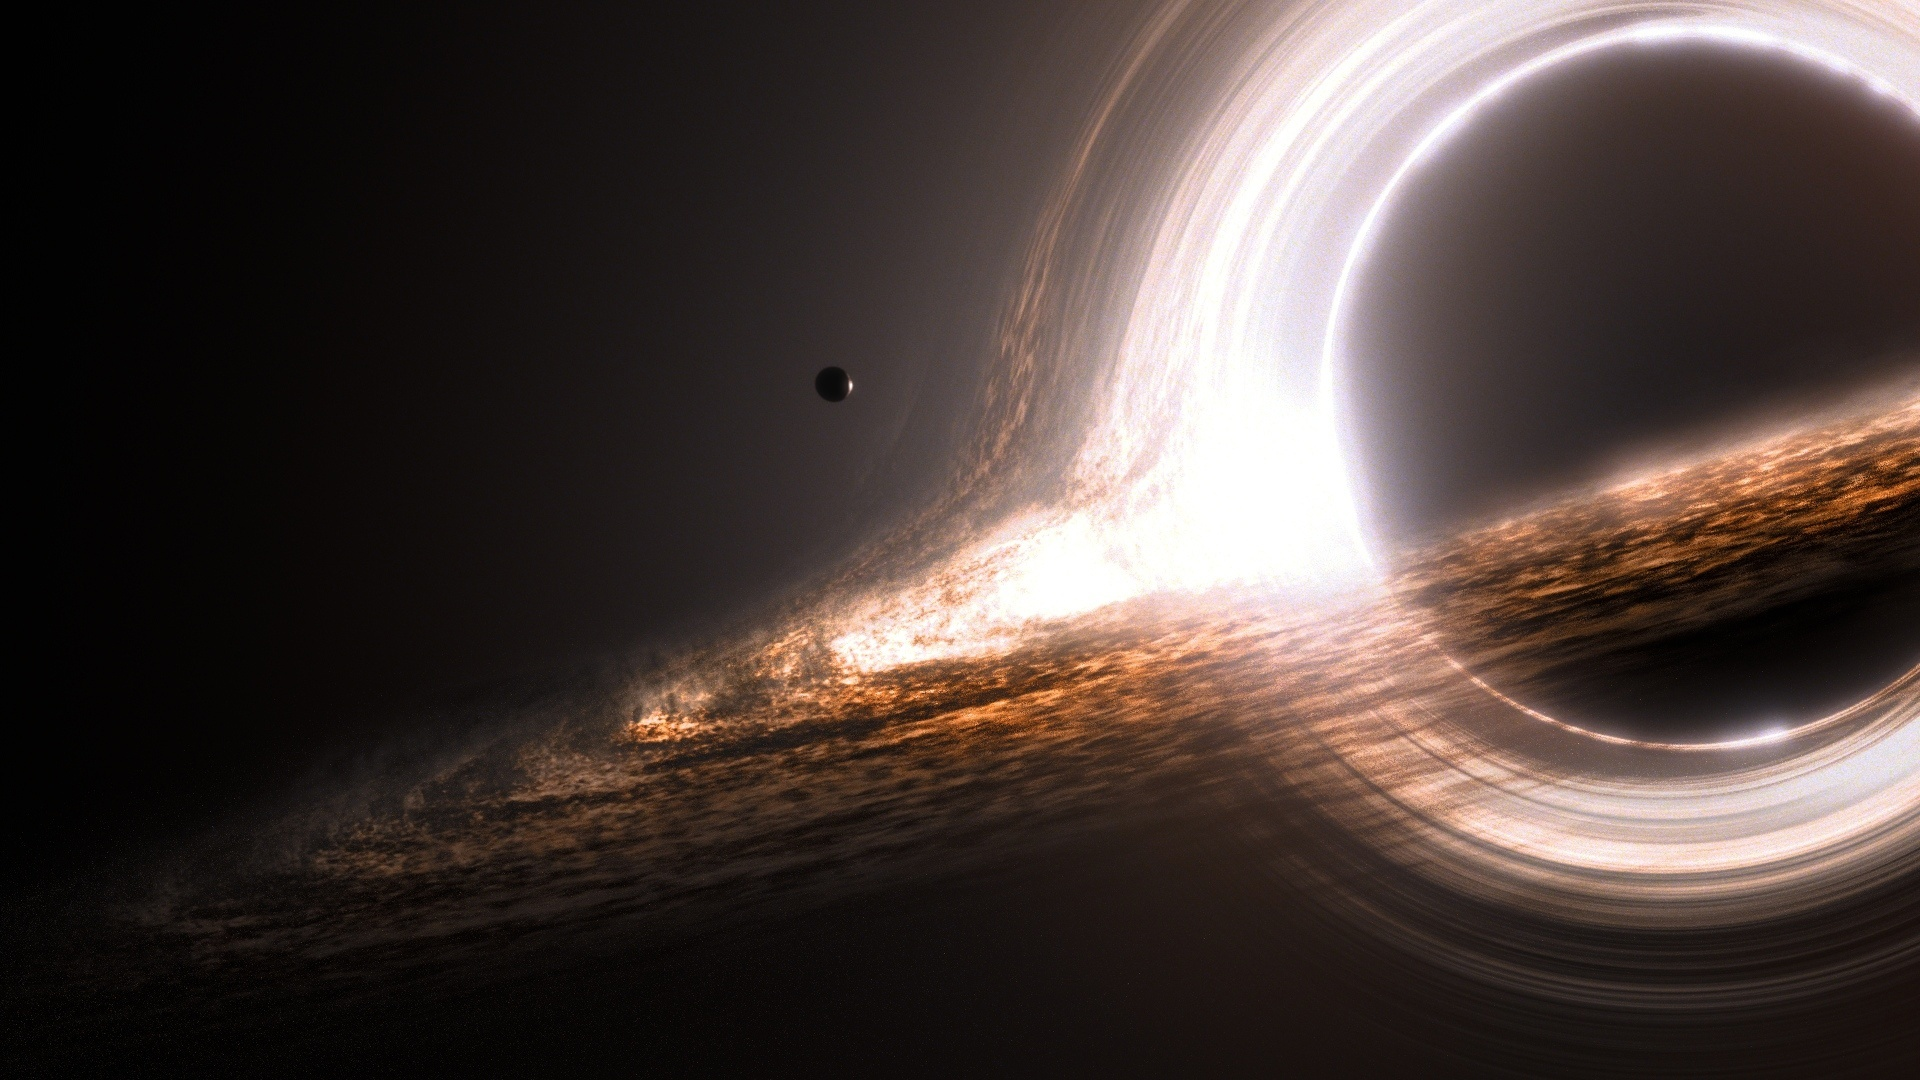
\includegraphics[height=\paperheight]{images/interstellar}}
\frame{\vspace*{12em}\titlepage}}
\frame{\tableofcontents}


\section[Gödel]{Gödels Unvollständigkeitssatz}

\begin{frame}
  \centering
  \bigskip

  \Huge \hil{Abschnitt I}

  \bigskip
  \Large\textbf{Gödels Unvollständigkeitssatz}
  \par

  \large

  Es gibt wahre Aussagen, die nicht beweisbar sind.

  \pause
  \bigskip
  \bigskip

  Zum Beispiel folgende:

  "`Diese Aussage ist nicht beweisbar."'
  \par
\end{frame}

\begin{frame}\frametitle{Vereinbarungen zur Metaebene}
  Auf der Metaebene wissen wir, \ldots
  \begin{enumerate}
    \item wie man mit endlichen syntaktischen Objekten operiert,

    \item was die natürlichen Zahlen sind,

    \begin{center}\begin{tikzpicture}
      \draw[-latex,dotted] (0.0,0) -- (5.5,0);
      \foreach \x in {0,1,2,3,4,5}
      \draw[shift={(\x,0)},color=black] (0pt,3pt) -- (0pt,-3pt);
      \foreach \x in {0,1,2,3,4,5}
      \draw[shift={(\x,0)},color=black] (0pt,0pt) -- (0pt,-3pt) node[below] {$\x$};
    \end{tikzpicture}\end{center}

    \item was es bedeutet, dass eine Zahl mit einer gewissen Eigenschaft
    existiert oder dass eine Behauptung für alle Zahlen stimmt.
  \end{enumerate}

  \pause

  Mögliche Wahlen der Metaebene:
  \begin{itemize}
    \item Gesunder Menschenverstand mit Platonismus
    \item Gesunder Menschenverstand mit Formalismus
    \item Diverse formale Systeme
  \end{itemize}
\end{frame}


\subsection[Beweisbarkeit und Wahrheit]{Beweisbarkeit und Wahrheit}

\begin{frame}{Beweisbarkeit und Wahrheit}
  \vspace*{-1em}
  \begin{block}{Syntaktisch}
  Eine Aussage~$A$ heißt genau dann \hil{beweisbar}, wenn es in einem
  fixierten formalen System einen \hil{formalen Beweis} von~$A$ gibt:
  \vspace*{-1em}
  \[ \PA \proves A \]
  \end{block}

  \begin{block}{Semantisch}
  Eine Aussage~$A$ heißt genau dann \hil{wahr}, wenn sie im
  \hil{Standardmodell} gilt:
  $\NN \models A$
  \end{block}
  
  \pause

  \begin{itemize}
    \item Jede beweisbare Aussage ist wahr.
    \item Nicht alle wahren Aussagen sind beweisbar.
    \item Es gibt \hil{Nichtstandardmodelle}:

    % https://boolesrings.org/victoriagitman/2015/04/22/an-introduction-to-nonstandard-models-of-arithmetic/
    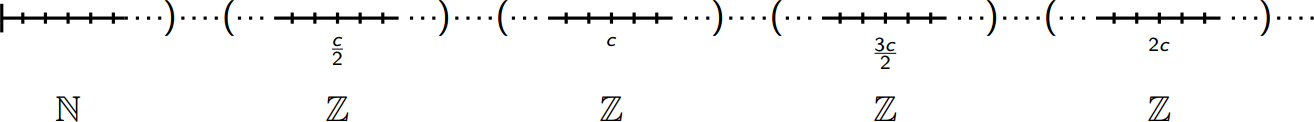
\includegraphics[scale=0.3]{nonstandard-model-of-arithmetic}
    % Tennenbaum 1959

    %\item In starker Metatheorie: Alle$^\star$ konsistenten formalen Systeme
    %besitzen
  \end{itemize}
\end{frame}


\subsection{Quines}

\begin{frame}{Quines}
  Wir schreiben~$\goedel{A}$ für die \hil{Gödelnummer} einer Aussage~$A$.

  \begin{block}{Reflexion von Beweisbarkeit}
    Es gibt eine Aussageform~$\Prov(n)$, sodass für jede Aussage~$A$
    genau dann~$\Prov(\goedel{A})$ wahr ist, wenn~$A$ beweisbar ist:
    \vspace*{-0.8em}
    \[ \NN \models \Prov(\goedel{A}) \quad\text{genau dann, wenn}\quad
      \PA \proves A. \]
  \end{block}
  \pause

  Mit dem \hil{Diagonallemma} gibt es eine Aussage~$A$ mit
  \vspace*{-0.2em}
  \[ \PA \proves (A \leftrightarrow \neg (\Prov(\goedel{A}))). \]
  \vspace*{-1em}
  \pause
  \justifying
  \begin{enumerate}
  \item Angenommen $\PA \proves A$. \pause
  Dann $\PA \proves \neg (\Prov(\goedel{A}))$, \pause
  also~$\NN \models \neg (\Prov(\goedel{A}))$, \pause
  also nicht~$\NN \models \Prov(\goedel{A})$, \pause
  also ist~$A$ nicht beweisbar, \pause
  also folgt ein Widerspruch.\pause
  \item Also ist~$A$ nicht beweisbar, \pause
  somit~$\NN \models \neg\Prov(\goedel{A})$.\pause
  \item Also~$\NN \models A$, d.\,h.~$A$ ist wahr.
  \end{enumerate}
\end{frame}


\subsection[Undefinierbarkeit]{Undefinierbarkeit von Wahrheit}

\begin{frame}{Undefinierbarkeit von Wahrheit}
  \begin{block}{Reflexion von Beweisbarkeit}
    Es gibt eine Aussageform~$\Prov(n)$, sodass für jede Aussage~$A$
    genau dann~$\Prov(\goedel{A})$ wahr ist, wenn~$A$ beweisbar ist:
    \vspace*{-0.8em}
    \[ \NN \models \Prov(\goedel{A}) \quad\text{genau dann, wenn}\quad
      \PA \proves A. \]
  \end{block}

  Kann man auch Wahrheit reflektieren? Gibt es eine Aussageform~$\True(n)$,
  sodass für jede Aussage~$A$ genau dann~$\True(\goedel{A})$ wahr ist, wenn~$A$
  wahr ist?
    \[ \NN \models \True(\goedel{A}) \quad\text{genau dann, wenn}\quad
      \NN \models A \]
  \pause

  \hil{Nein:} Mit dem Diagonallemma gäbe es eine Aussage~$A$ mit
  \[ \PA \models (A \leftrightarrow \neg(\True(\goedel{A}))). \]
  Zu deutsch besagte~$A$: "`Aussage~$A$ ist nicht wahr."'
  Diese Aussage wäre genau dann wahr, wenn sie nicht wahr ist.
\end{frame}


\subsection[Konsistenz]{Konsistenzreflexion}

\begin{frame}{Konsistenzreflexion}
  Sei~$A$ die Aussage~"`Aussage~$A$ ist nicht beweisbar"':
  \[ \PA \proves (A \leftrightarrow \neg (\Prov(\goedel{A}))). \]

  \begin{block}{Resultat von Gödel--Rosser}
    Auch ohne die Unterstellung der Existenz von~$\NN$ in der Metatheorie gilt:
    Ist~$\PA$ konsistent (d.\,h. ist~$1 = 0$ nicht beweisbar),
    so ist~$A$ nicht beweisbar.
  \end{block}
  \pause

  Da sich der Beweis dieses Resultats formalisieren lässt, folgt
  \[ \PA \proves (\neg(\Prov(\goedel{1 = 0})) \rightarrow
  \neg(\Prov(\goedel{A}))). \]

  \justifying
  Angenommen~$\PA \proves \neg(\Prov(\goedel{1 = 0}))$. Dann~$\PA
  \proves \neg(\Prov(\goedel{A}))$, das ist falsch. Somit kann~$\PA$ seine
  Konsistenz nicht beweisen.
\end{frame}


\section[Halteproblem]{Das Halteproblem}

\begin{frame}
  \centering
  \bigskip

  \Huge \hil{Abschnitt II}

  \bigskip
  \Large\textbf{Spiel und Spaß mit \\ Berechenbarkeitstheorie}
  \par
  \bigskip
  \bigskip

  \centering
  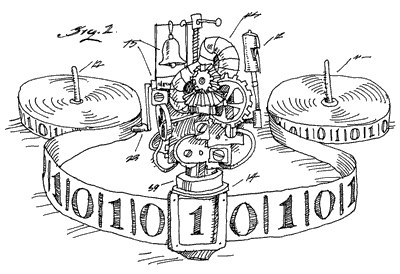
\includegraphics[scale=0.4]{turing-machine}
  \par
\end{frame}


\subsection[Unentscheidbarkeit]{Unentscheidbarkeit des Halteproblems}

\begin{frame}{Unentscheidbarkeit des Halteproblem}
  Ein \hil{Halteorakel} ist ein Programm, dass ein Programm~$P$ als Eingabe liest
  und korrekt ausgibt: "`$P$ hält"' oder~"`$P$ hält nicht"'.
  \bigskip
  \pause

  Wenn es ein Halteorakel gäbe, könnte man auch folgendes Programm~$Q$
  entwickeln:
  \code{
    Befrage das Halteorakel, ob Programm~$Q$ hält.

    Falls ja: Dann gehe in eine Endlosschleife.

    Falls nein: Dann halte.
  }
  \pause
  Das Programm~$Q$ hält genau dann, wenn es nicht hält.
  \bigskip

  Ein Halteorakel gibt es nicht.
\end{frame}


\subsection[Unabhängigkeit]{Unabhängigkeit}

\begin{frame}{Ein Programm mit unbeweisbarem Halteverhalten}
  Wir betrachten folgendes Programm~$P$:
  \code{
    Laufe systematisch alle formalen Beweise ab.
    Sobald ein Beweis von~$1 = 0$ gefunden wurde, halte.
  }
  \pause

  \begin{itemize}
    \item Das Programm~$P$ hält nicht.
    \item Die Aussage, dass~$P$ nicht hält, ist in~$\PA$ nicht beweisbar.
    \pause
    \item Sei~$n$ die Anzahl Zustände, die eine Umsetzung von~$P$ als
    Turingmaschine benötigt. Dann entzieht sich~$\mathrm{BB}(n)$ der
    Beweisbarkeit in~$\PA$.
  \end{itemize}
\end{frame}


\subsection{Das universelle Programm}

\begin{frame}{Das universelle Programm}
  Wir betrachten folgendes Programm~$P$:
  \code{
    Laufe systematisch alle formalen Beweise ab.
    Sobald ein Beweis einer Aussage der Form
    "`Die Ausgabe von Programm~$P$ ist nicht die Liste
    $x_1,\ldots,x_n$"'
    gefunden wurde, gib die Liste~$x_1,\ldots,x_n$ aus und halte.
  }

  \begin{enumerate}
    \item $\PA$ beweist, dass~$P$ eine endliche Liste von Zahlen ausgibt.
    \item Für jede endliche Liste von Zahlen gibt ein
    Universum~$M$, sodass~$P$ genau diese Liste ausgibt, wenn man es in~$M$
    ausführt.
  \end{enumerate}
\end{frame}


\section[Zufall]{Randomisierte Strategien}

\begin{frame}
  \centering
  \bigskip

  \Huge \hil{Abschnitt III}

  \bigskip
  \Large\textbf{Zufall als wertvolle Ressource}
  \par
  \bigskip
  \bigskip

  \centering
  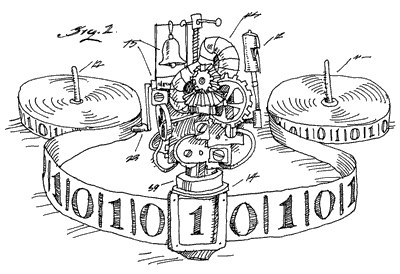
\includegraphics[scale=0.4]{turing-machine}
  \par
\end{frame}
\begin{frame}{Welche Zahl ist größer?}
  Alice denkt sich zwei verschiedene reelle Zahlen~$x$ und~$y$ aus und verstaut
  sie in undurchsichtigen Boxen:
  \begin{center}
    \kasten{} \qquad \kasten{}
  \end{center}
  Bob darf in eine der Boxen hineinschauen und darf dann einen Tipp abgeben,
  welche der Zahlen größer ist.
  \bigskip

  \justifying
  Es gibt eine \hil{randomisierte Strategie}, mit der Bobs
  Gewinnwahrscheinlichkeit bei jeder Wahl
  von~$x$ und~$y$ mehr als~$50\,\%$ beträgt.
  \bigskip
  \pause

  \begin{center}\begin{tikzpicture}
    \draw (-3.0,0) -- (3.0,0);
    \foreach \x in {-2,0.5,2}
      \draw[shift={(\x,0)},color=black] (0pt,3pt) -- (0pt,-3pt);
    \draw[shift={(-2,-0.4)},color=black] node {$x$};
    \draw[shift={(0.5,-0.4)},color=black] node {$r$};
    \draw[shift={(2,-0.4)},color=black] node {$y$};
  \end{tikzpicture}\end{center}
  
  \par
\end{frame}


\end{document}
